\documentclass{article}

\usepackage{amssymb}
\usepackage{amsfonts}
\usepackage{amsmath}
\usepackage[margin=1in]{geometry}
\pagestyle{empty}

\newtheorem{thm}{Theorem}[section]
\newtheorem{conj}[thm]{Conjecture}
\usepackage{graphicx}
\usepackage{epstopdf}
\usepackage{wrapfig}
\usepackage{float}
\begin{document}	
\noindent 80977816 \hspace{5.5in} 4/3/17\\

\begin{enumerate}
	\item Let $T(i)$ be the expected number of moves to reach $n$ starting from position $i$ using this reflecting boundary. $T(n) = 0$, because if we're at $n$ there's no where to go. If $0<i<n$, $T(i) = \frac{1}{2}T(i-1) + \frac{1}{2}T(i+1)+1$ because at location $i$ we can go to $i-1$ or $i+1$ with equal probabilities and that takes 1 step.  If $i=0$ either on the next step we go to $i=1$ or we stay at $i=0$, each with probability $\frac{1}{2}$.  Therefore, $T(0)=\frac{1}{2}T(1)+\frac{1}{2}T(0)+1$, which means that $T(0)=T(1)+2$.\\\\
	So the full recurrence relation is: \\
	$
	T(i) = 
	\begin{cases}
	0 & i = n \\
	T(1) + 2 & i = 0 \\
	0.5T(i+1) + 0.5T(i-1) + 1 & \textup{otherwise} \\
	\end{cases}
	$
	\\\\
	Now examining the explicit form of the solution to the recurrence found in class and after computing out this recurrence relation for $n=4$, suppose that $T(i) = n^2+n-i^2-i$.  I'll show that this explicit form hold by induction.  \\
	The base cases are $i = 0$ and $i = n$.  \\
	$T(n) = n^2 + n - n^2 - n = 0$, which is correct \\
	$T(0) = n^2 + n$ and $T(0) = T(1) + 2 = n^2 + n - 1 - 1 + 2 = n^2 + n$, and so the base cases hold.  \\
	$T(i) = 0.5T(i-1) + 0.5T(i+1) + 1  \\
		  = 0.5(n^2+n-(i-1)^2-(i-1))+0.5(n^2+n-(i+1)^2-(i+1))+1 \\
		  = n^2 + n - 0.5(i^2-2i+1)-0.5(i-1)-0.5(i^2+2i+1)-0.5(i+1)+1 \\
		  = n^2 + n - i^2 - 1 - i + 1 \\
		  = n^2 + n - i^2 - i $ and so the induction holds and the explicit formula $T(i) = n^2 + n - i^2 - i$ is valid.  \\
	\\
	The solution we found in class without the reflecting boundary was $T(i) = n^2 - i^2$ which is less than the value that was just found with the non-reflecting boundary. It makes sense that this variation on the problem will take longer than the one in class because it's possible to stay at zero for an indefinite amount of time.    
	
	\item The maximum flow value is 8 and so is the final value of the cut.  These are the final flow values down each edge: $(s,a) \to 4, 
	 (a,b) \to 3,
	 (a,d) \to 0,
	 (a,e) \to 1,
	 (b,t) \to 3, 
	 (e,t) \to 2,
	 (s,c) \to 4,
	 (c,a) \to 0,   
	 (c,d) \to 3,
	 (c,e) \to 1,
	 (d,t) \to 3
	$ \\
	The edges that cross the cut are $(c,e), (a,e), (a,b),$ and $(d,t)$\\\\
	In the image below, the networks in the right column represent the residual netwrok at each iteration of the algorithm and to the right of those is the newest augmenting path that has been found.  The left column of networks shows how much flow is currently going down each edge in the original graph.  For example, 4/5 indicates that 4 units of flow are passing down an edge that can hold at most 5 units of flow.  
	
	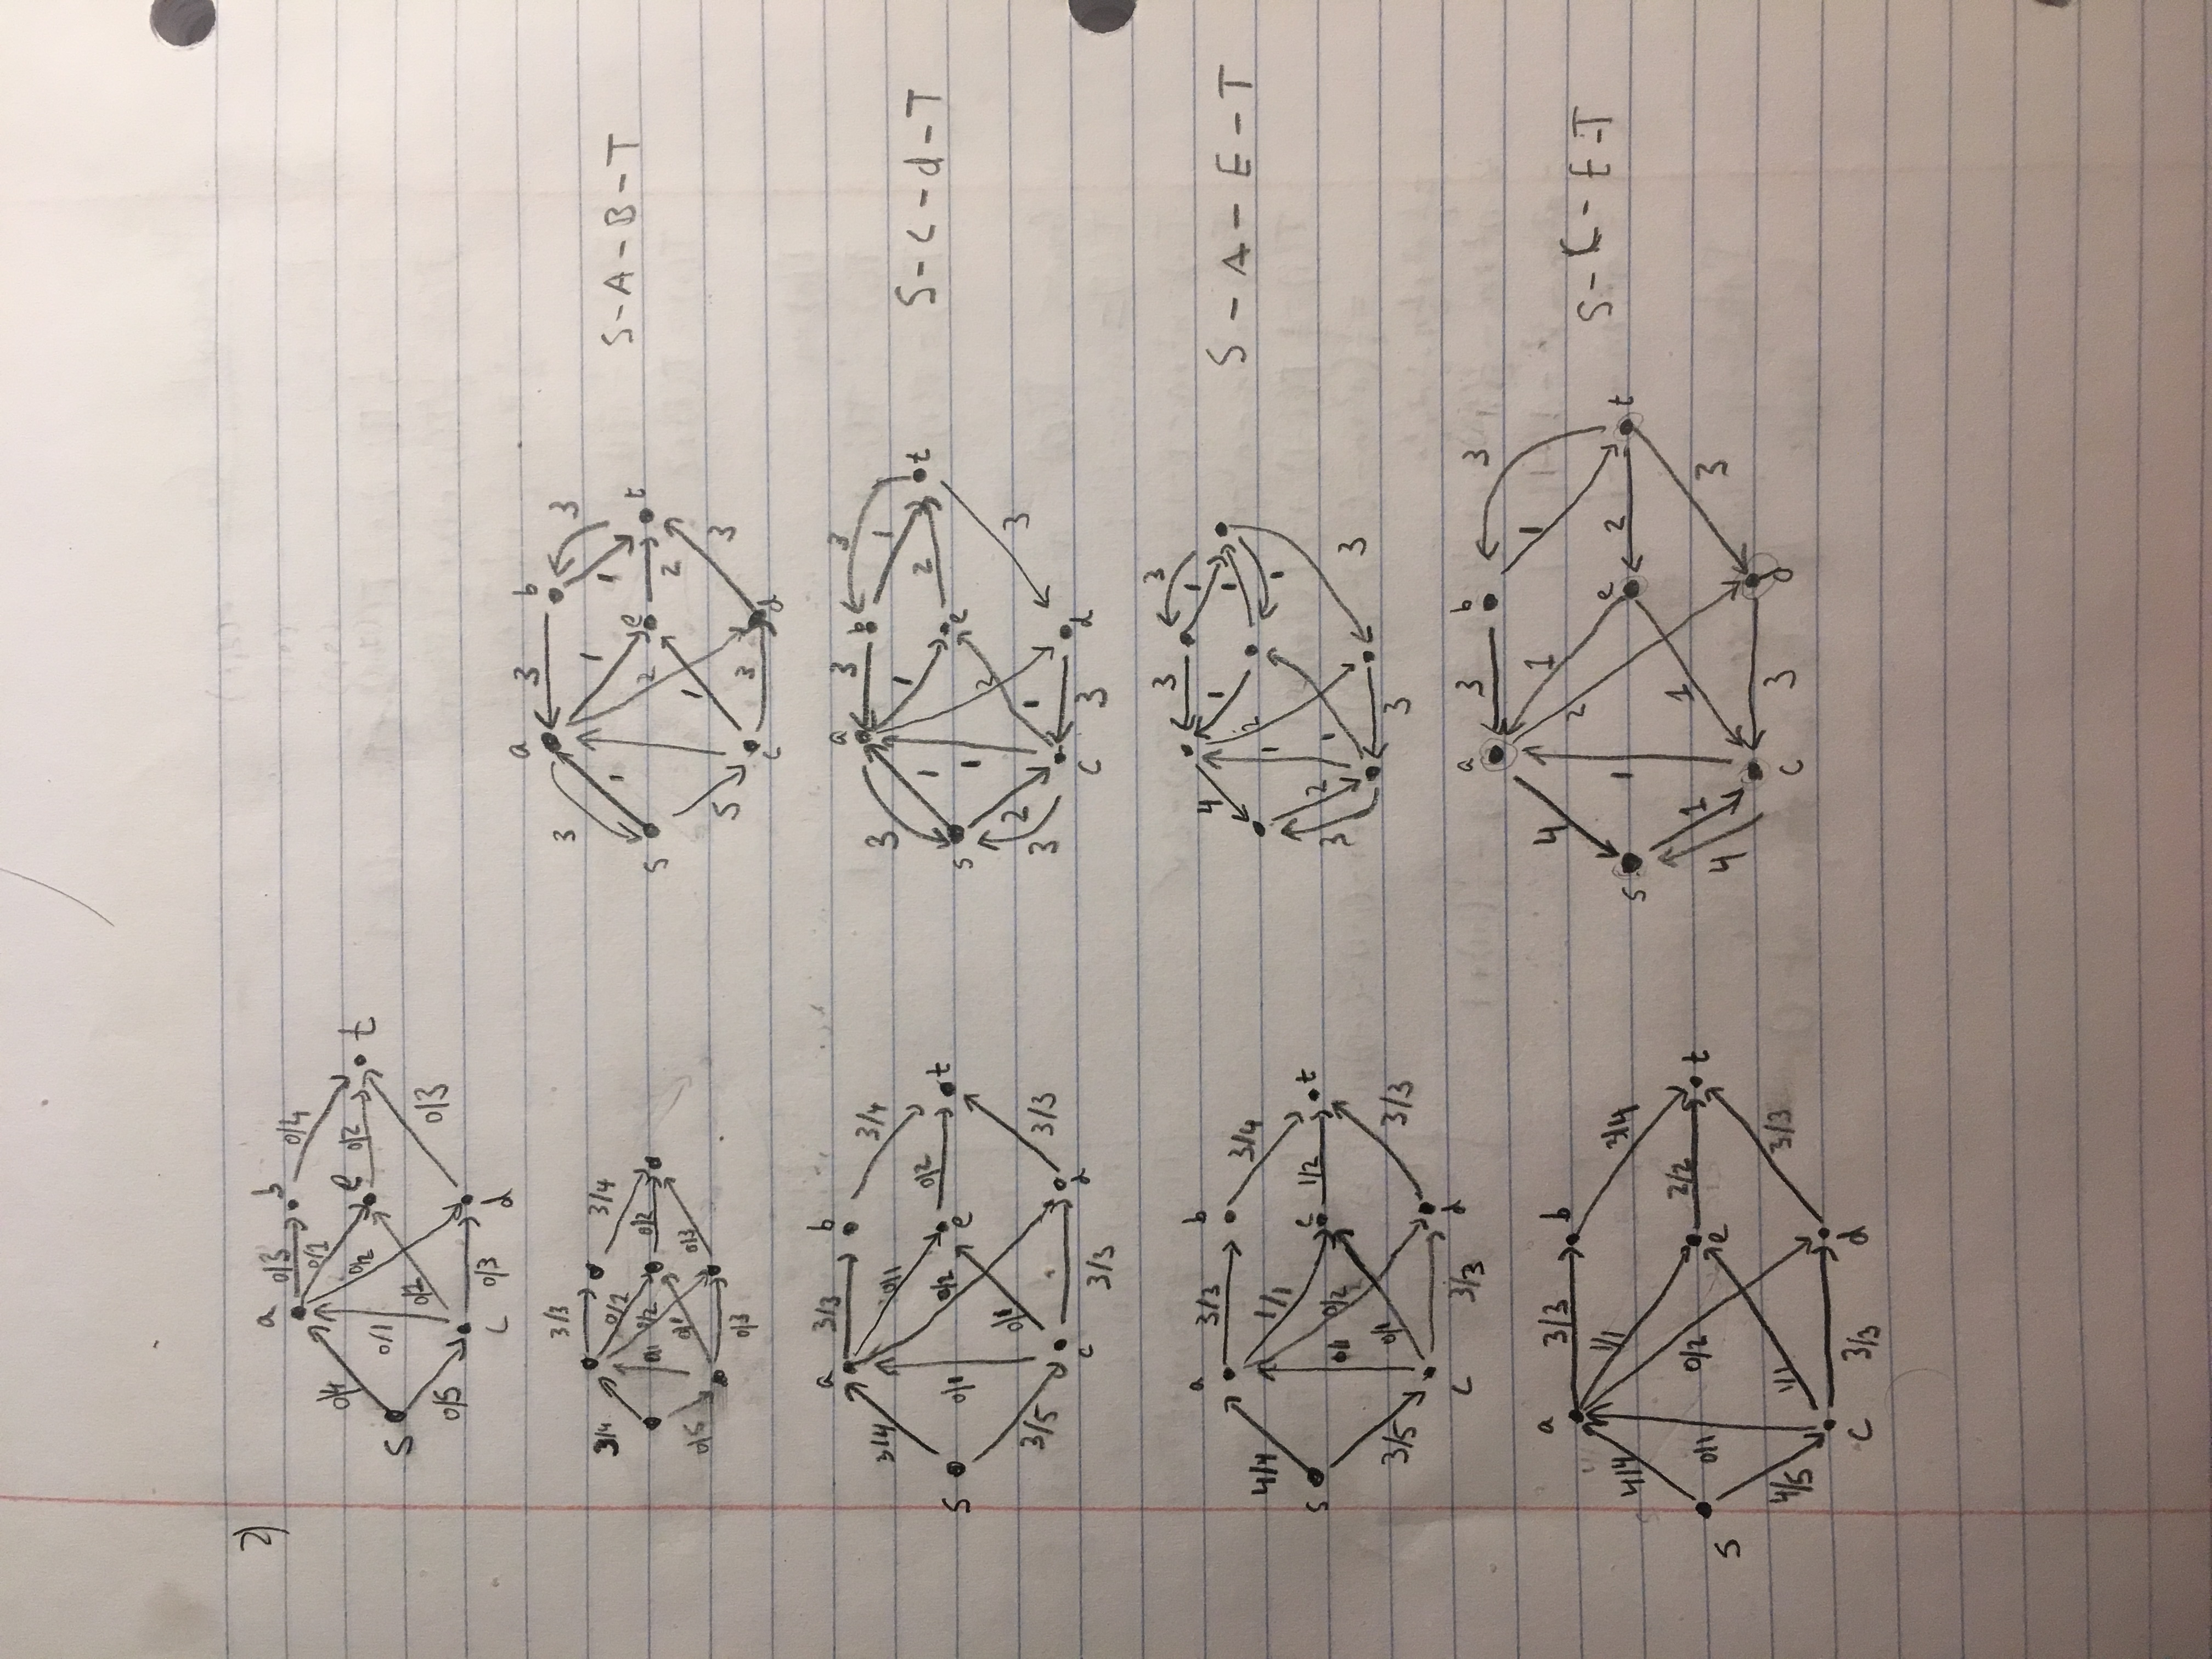
\includegraphics[scale=.1, angle = -90]{Question_2.JPG}
	
	\item First do one pass over the $n\times n$ array of land to find the column or row that can sustain the fewest number of palm trees.  Call this number $p$.  Because every row and every column contains at least $p$ subplots that can sustain a palm tree, there must exist some solution in which every column and every row contains exactly $p$ palm trees.  To find this configuration, I'm going to reduce (convert) this problem to a network flow problem and then show that the maximum flow of this network will correspond to a valid solution to this palm tree problem.  \\\\
	
	In the graph that will correspond to an given plot of land, create $n$ vertices $r_1, r_2,...r_n$ to correspond to the rows of this plot of land, $n$ more vertices $c_1, c_2, ... c_n$ for the columns, and then a source vertex $s$ and a sink $t$.  Now construct edges $(s, r_i)$ for all $i$ with capacity $p$, edges $(c_j, t)$ also with capacity $p$ for all $j$, and add edge $(r_i, c_j)$ with capacity 1 if and only if the subplot in position $(i,j)$ in the plot can sustain a palm tree. So this graph has $2n+2$ vertices and in the worst case $n^2 + 2n$ edges.  The flow through this network corresponds to the number of palm trees that can be planted in this array and if we have some flow through network (any flow, not even the max necessarily), we can convert this to a palm tree planting arrangement by examining which of the edges $(r_i, c_j)$ have a flow of 1 going through them. By construction, the maximum possible value the maximum flow could take on is $n\cdot p$ (though it hasn't yet been shown that this is actually the maximum flow).  \\\\
	
	Now here's why if the Ford-Fulkerson algorithm is run on this network, it will show that the maximum flow of this network is $n\cdot p$ and will generate a valid palm tree planting in which there are the same number of trees in every row and every column.  Because the total capacity $p$ that enters any row vertex must be less than or equal to the sum of the capacities that leave it by the definition of $p$, we will always be able to push $p$ amount of flow through each $r_i$ and as a result, since the sum of the capacities entering each column vertex is greater than the outgoing capacity also equal to $p$, we can push $p$ through each column to $t$ and ultimately this ensures that exactly $p$ palm trees are in every row and column and so the maximum flow (and thus the maximum number of palm trees) is $n\cdot p$.  \\
	
	The Ford Fulkerson Algorithm using BFS runs in $O(VE^2)$ time which in this case is the same as $O((2n+2)(n^2+2n)^2) = O(n^5)$.  Using DFS, it runs in $O(Ef^*)$, where $f^*$ is the maximum flow and so in this case using DFS will lead to a $O((n^2+2n)np) = O(n^3p)$ runtime.  $p$ can be as large as $n$, if all the rows can support $n$ palm trees that is and so the asymptotic runtime of this would be $O(n^4)$.  	
	\item
	\begin{enumerate}
		\item For this problem there are two sorts of constraints we need to include in the linear program, the capacity constraints and the flow loss constraint.  \\
		Let $f_{ij}$ be the flow from node $i$ to $j$ and let $c_{ij}$ be the capacity of the connection between node $i$ and node $j$.  \\
		Therefore, for all edges $(i,j)$ in the graph, add the constraint $0 \leq f_{ij} \leq c_{ij}$\\
		Then for every vertex $v$ except $s$ and $t$, add this flow loss constraint: $\displaystyle\sum_{(i,v)\in E}f_{iv} = 2\sum_{(v,j)\in E}f_{vj}$, which encodes the fact that half the flow is lost at every vertex.  \\
		Because we want to maximize the flow, let the objective function be $\displaystyle\max\sum_{(k,t)\in E}f_{kt}$, the amount of flow that enters $t$.  This is equivalent to maximizing the amount of flow that leaves $s$.  
		
		\item To find the maximum flow configuration with the minimum cost, I'll run two linear programs.  The first one will calculate the maximum flow through a network and then the second will minimize the cost of a flow configuration with the maximum flow.  \\
		For the first problem add capacity constraints $0\leq f_{ij} \leq c_{ij}$ for all edges $(i,j)$ in the network and conservation of flow constraints which say that the flow going into a vertex equals the flow leaving that vertex for all vertices $v$ except vertices $s$ and $t$: $\displaystyle\sum_{(i,v)\in E} f_{iv} = \sum_{(v,j)\in E}f_{vj}$.  \\
		We want to maximize the flow leaving $s$ and so the objective function which we want to maximize is $\displaystyle\sum_{(s,i) \in E}f_{si}$.  Run this first linear program with these constraints to find the maximum flow of the network, which shall be called $M$.  \\
		\\
		Now to find the minimum cost and maximum flow configuration, use the same capacity and conservation of flow constraints as before and add this constraint which says that the flow must always be $M$: $\displaystyle\sum_{(s,i) \in E}f_{si} = M$.  In other words that the total flow leaving vertex $s$ must always be $M$.  \\
		The objective function which we want to minimize is now $\displaystyle\sum_{(i,j) \in E}f_{ij} \cdot c_{ij}$, where $c_{ij}$ is the unit cost of flow through edge $(i,j)$. \\
		So using these constraints and minimizing this objective funciton will allow us to find the maximum flow with the minimum cost for a given network.   
	\end{enumerate}
	
	\item If we're given the maximum flow value of a graph as well as all the flow assignments to every edge in the graph, we can calculate the residual graph for $G$.  When the Ford-Fulkerson algorithm has been run to completion, the residual graph has been partitioned into two sets of vertices $S$ and $V-S$, where $S$ contains $s$ and all the vertices that can be reached from $s$ and where $V-S$ contains the rest, including $t$. If at the end of Ford-Fulkerson, $t$ could be reached from $s$ in the residual graph, then it would be possible to send more flow from $s$ to $t$ and thus Ford-Fulkerson couldn't have found the maximum flow and been run to completion, a contradiction. Therefore, when a network has the maximum amount of flow going through it, in the residual graph, there is no path from $s$ to $t$. For both of the following parts, compute the residual graph before updating the edge $e$
	\begin{enumerate}
		\item If the capacity of a given edge $e$ is increased by 1, check the residual graph to see if the flow through $e$ was equal to its capacity.  If it was not and it already had some residual capacity, then the maximum flow of the graph will be unchanged - adding more residual capacity to an edge won't change the maximum flow because if it did, that residual capcity would've already been used.  Now, if the edge was previously at had no residual capacity and now has had 1 unit of residual capacity, run one round of either DFS or BFS starting from $s$ (both take $O(|V| + |E|)$ time) to see if there is now a path (that goes through $e$) to $t$.  If there is such a path then 1 unit of flow can be sent along it and the new maximum flow is 1 larger than it was before.  We can then do one last pass over the edges in this path to update the amount of flow going through them.  If there is no path, return the original maximum flow.  We only have to do one round of updating the edges (assuming there is a path) because once we've updated the flow through edge $e$ we've reached a new maximum configuration and there cannot be any other paths through the residual graph.  
		
		\item Now if we decrease the weight of $e = (u,v)$ by 1, again check the residual graph.  If $e$ originally had residual capacity and we decrease the residual capacity of $e$ nothing will change.  If $e$ had no residual capacity, one of two things could happen - either one unit of flow through $e$ is rerouted through some other channels, in which case the maximum flow does not change, or it cannot be rereouted and the maximum flow decreases by 1.  To see if we can 'reroute' this flow, run a BFS or DFS in the residual graph (with $e$'s updated capacity) from $u$ to see if there is a path from $u$ to $v$ and that doesn't take edge $e$, because edge $e$ is now at capacity since the capacity was decreased by 1.  If there is an alternative path from $u$ to $v$, then we can update the edges along that path to take one more unit of flow (a path like this could definitely exist because there can be multiple configurations that lead to the maximum flow).  This takes $O(|V|+|E|)$ time to do the graph traversal and path updating. If this path exists, the maximum flow is unchanged. If there isn't a path from $u$ to $v$, the maximum capacity of the graph has been reduced and so we need to find a path from $s$ to $u$ and decrease the flow along those edges and also find a path from $v$ to $t$ and decrease the flows along those edges to reflect this change.  
	\end{enumerate}
	
	\item 
	\begin{enumerate}
		\item Let $x_1, x_2, x_3, x_4$ be the probabilities the row player plays strategies 1,2,3 and 4 respectively.  \\
		Because these are probabilities they're between 0 and 1: $0\leq x_1, x_2, x_3, x_4$ and $x_1 + x_2 + x_3 + x_4 = 1$ \\
		The objective function is $\displaystyle\max z$ and the other contstraints are: \\
		$3x_1+6x_2-3x_3-7x_4 \geq z \\
		x_1-2x_2-2x_3+4x_4 \geq z \\
		0x_1-2x_2+3x_3-5x_4 \geq z \\
		-4x_1+0x_2-3x_3+7x_4 \geq z \\
		$
		\\\\
		Let $y_1, y_2, y_3, y_4$ be the probabilities the row player plays strategies 1,2,3 and 4 respectively.  \\
		Because these are probabilities they're between 0 and 1: $0\leq y_1, y_2, y_3, y_4$ and $y_1 + y_2 + y_3 + y_4 = 1$ \\ 
		The objective funciton is $\displaystyle\min w$ and the other constraints are: \\
		$3y_1+y_2+0y_3-4y_4 \leq w \\
		6y_1-2y_2-2y_3+0y_4 \leq w \\
		-3y_1-2y_2+3y_3-3y_4 \leq w \\
		-7y_1+4y_2-5y_3+7y_4 \leq w \\
		$
		
		\item Using an LP solver, I found that $z = -0.384, x_1 = .151, x_2 = .276, x_3 = .379, x_4 = .194\\
		w = 0.384, y_1 = .139, y_2 = .208, y_3 = .401, y_4 = .252$ \\
		
		\item The value of the game is 0.384. The column player should pay the row player 0.384 to make the game fair.  
	\end{enumerate}
\end{enumerate}

\newpage
I collaborated with Lauren Kim and Manav Khandewal on this pset.  
\end{document}
